\chapter{Related Work}  \label{chap:three}%

This chapter provides an overview of the related literature. Firstly, \Cref{sec:mono3d} provides a concise summary of prior works on the Providentia Mono3D System. Following this, \Cref{sec:instance_segmentation_models} delves into the task of instance segmentation, introducing state-of-the-art deep learning models utilized for this task. These models are presented within a hierarchical taxonomy, offering insight into their categorization and methodologies. In particular, two state-of-the-art (SOTA) instance and amodal instance segmentation models, YOLOv8 and Coarse-to-Fine Segmentation (C2F-Seg), which are exploited in this work, are introduced in deeper detail in this section. 

\section{Providentia Mono3D System}  \label{sec:mono3d}

The Providentia Monocular 3D Perception task (Mono3D) describes the process of detecting three-dimensional objects from a single two-dimensional RGB camera output frame. This Mono3D toolchain is described in the works “Real-Time Monocular 3D Object Detection to Support Autonomous Driving” by Leon Blumenthal \cite{thesisLeon} and “Monocular 3D Object Detection Using HD Maps” by Joseph Birkner \cite{thesisJoseph}. In \cite{thesisLeon}, the Providentia Mono3D detecter splits the detection task into two separate steps: a 2D instance segmentation step and a 3D lifting step. This so-called two-stage detection model is adapted and refined in the thesis of Joseph  \cite{thesisJoseph}. The first work focused on highway scenarios, where the yaw value (the direction of travel) is fixed. The second work addressed and generalized to the more urban scenarios where the yaw value is variable. The proposed approach was then evaluated on the TUM Traffic Intersection Dataset. This dataset has been covered in detail in \Cref{section:TUMTrafIntersectionDataset}. 

For each object, Mono3D estimates the basic 3D perception values, including birds-eye-view (BEV) positions $X/Y$, BEV size $L/W$, object height $H$, and headling angle (yaw) $\theta$. The elevation of the object over the road surface $Z$, pitch $\phi$, and roll $\gamma$ values are set to 0 always. Along with these basic values, Mono3D also provides an identifier for the object across multiple frames $I$,  the planar speed $\delta$$X/$$\delta$$Y/$$\delta$$Z$, and category $C$. These make up a total of fourteen dimensions in the output, as shown in \Cref{tab:mono3dOutputVariables}. 

\begin{table}[htb]%
	\centering%
	\begin{tabular}{ll}
		\toprule
		\textbf{Variable}  & \textbf{Description}  \\
		\midrule
		$X/Y$ & Position along the longitudinal/lateral axes  \\
		$Z$ & The elevation of the object over the road surface ($=0$)\\
		$L/W/H$ & Length/Width/Height of the object \\
		$\gamma/\phi/\theta$ & Roll/Pitch/Yaw angles, yaw determines travel direction ($\gamma=0, \phi=0$) \\
		$C$ & category \\
		$I$ & Object Identifier across multiple frames \\
		$\delta$$X/$$\delta$$Y/$$\delta$$Z$ & Derivatives of the position variables := speed  \\
		\bottomrule
	\end{tabular}
	\caption{The fourteen-dimensional output of Mono3D per object}
	\label{tab:mono3dOutputVariables}%
\end{table}

The Mono3D detection flow consists of three process nodes as shown in \Cref{mono3D architecture}: a camera driver node, a 2D instance segmentation node, and a 3D detection node. The 2D instance segmentation node continuously receives full-resolution $1920x1200$ RGB frames from the camera driver node. This communication exploits the Enhanced Communication Abstraction Layer (eCAL) \cite{ecal} shared memory as middleware for throughput and high performance. The second node exploits the YOLOv7 \cite{yolov7} instance segmentation model for detection and publishes an array of detections containing a confidence score, a category, a 2D bounding box, and a per-pixel instance mask to downstream processes via Robot Operating System (ROS) \cite{ros}. The 3D detection node subscribes to the instance segmentation node, receives the 2D instance detections, and starts with the so-called 3D lifting stage. This stage adapts and develops the L-Shape Fitting Method for Vehicle Pose Detection from LiDAR \cite{lsf} using HD map and tracking algorithm to stabilize the 3D detections and speed estimations. The currently chosen tracking algorithm is Simple Online and Realtime Tracking (SORT) \cite{sort}, a lightweight tracking algorithm specifically designed for real-time applications. Finally, the final fourteen-dimensional output of the entire flow is published via ROS to downstream applications, such as sensor fusion, visualization, or autonomous vehicles.

\begin{figure}[htb]%
	\centering%
	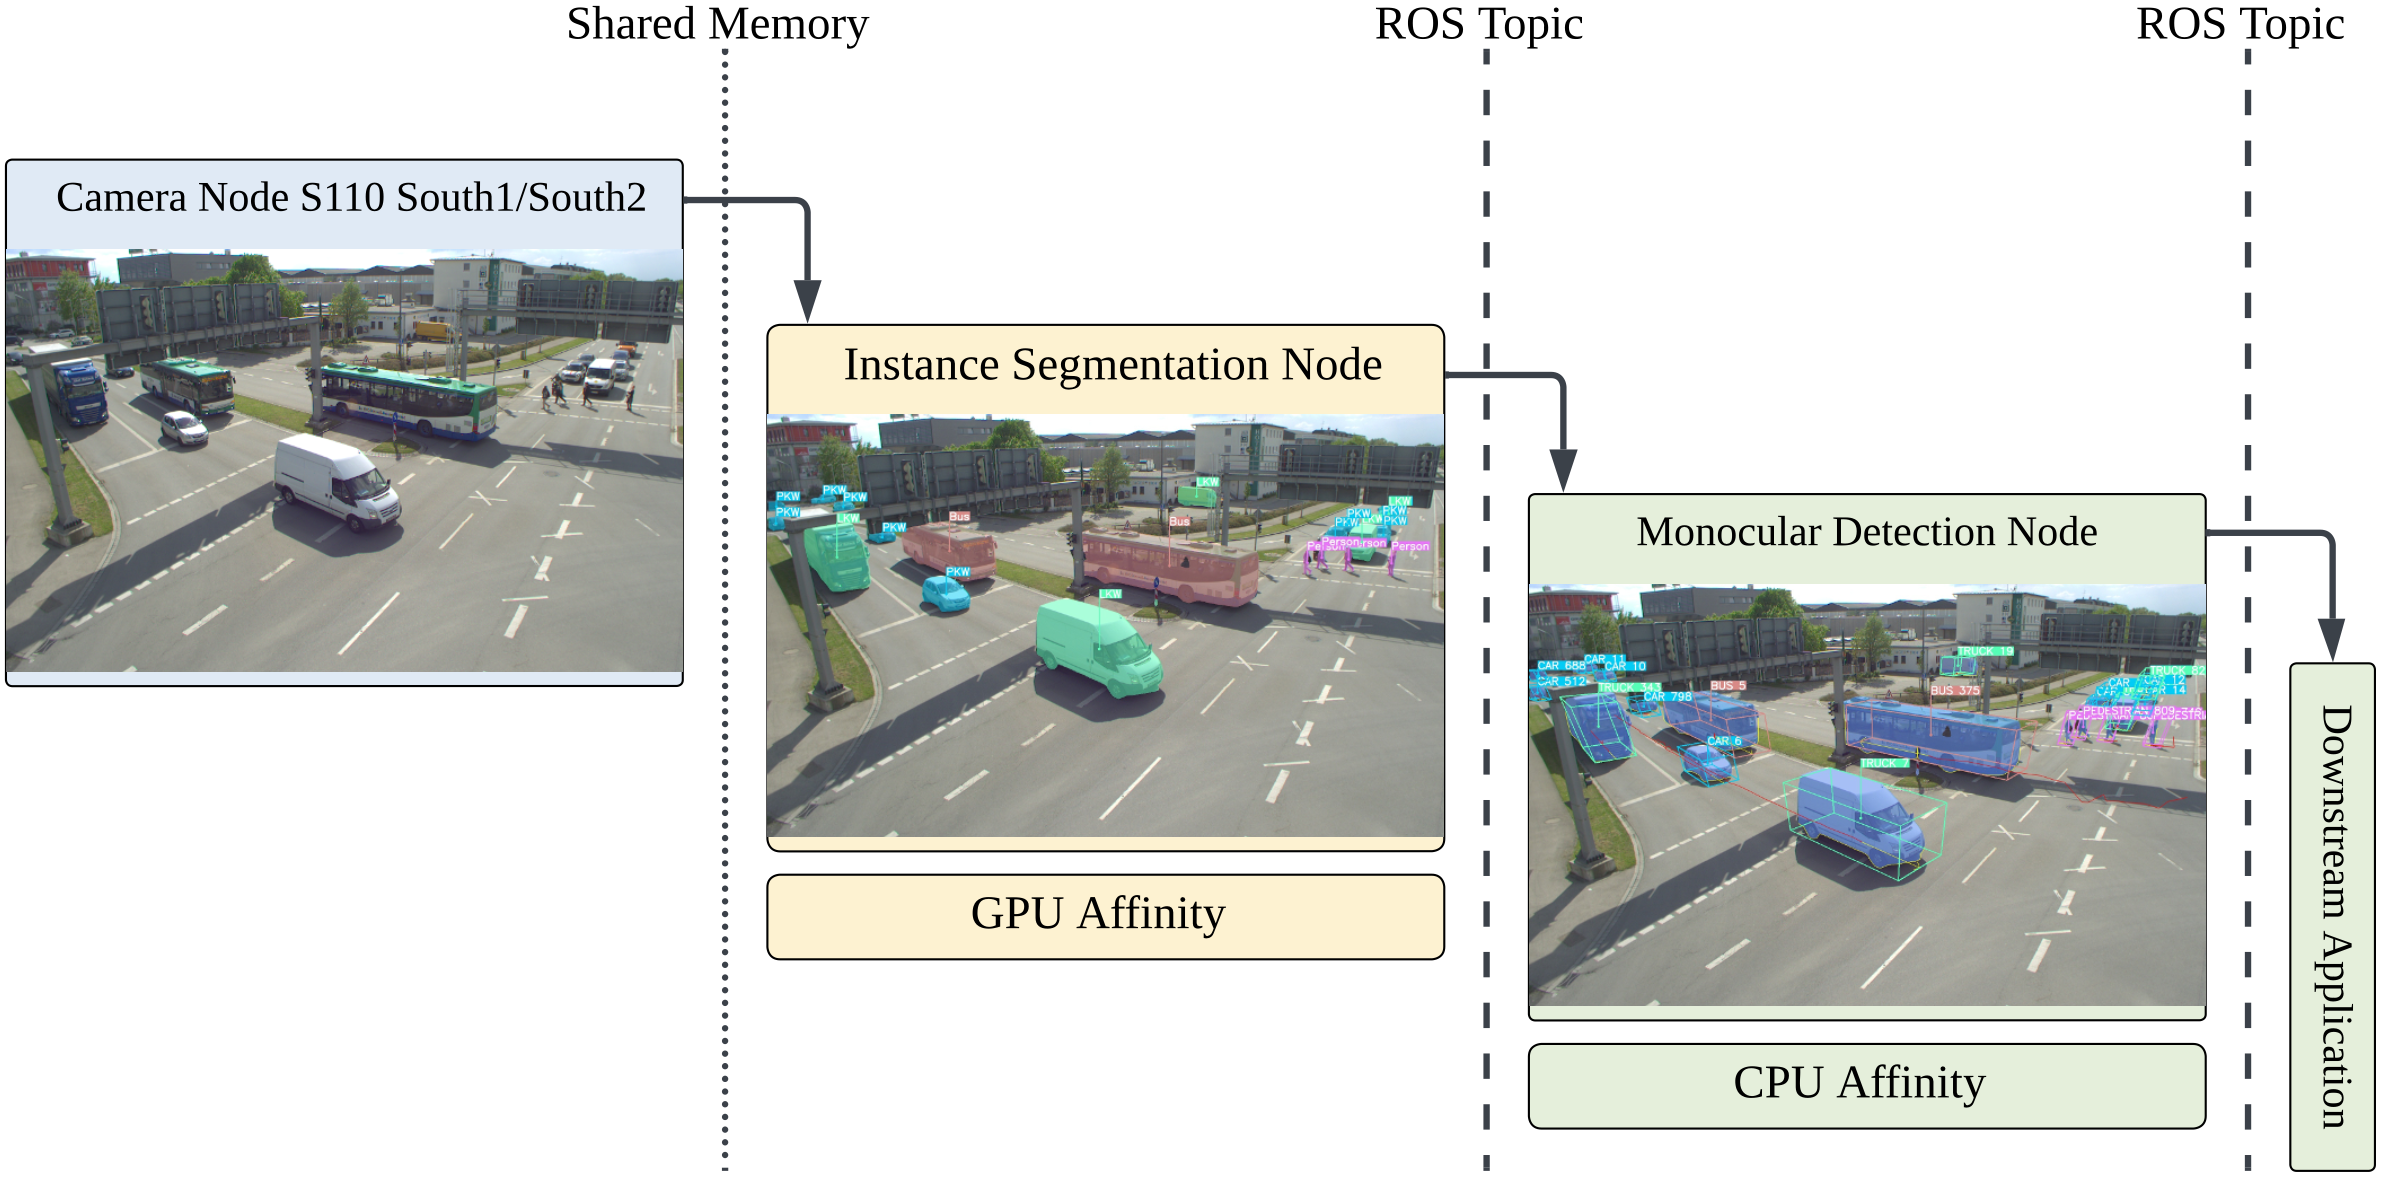
\includegraphics[width=150mm]{figures/mono3D-architecture.png}%
	\caption{Providentia Mono3D system architecture from \cite{thesisJoseph}. The camera driver publishes frames to Shared Memory, which are picked up from the instance segmentation node. The 2D detections from each frame are published to the Monocular Detection Node through ROS. The final 3D perception outputs are then published via ROS to downstream applications.}%
	\label{mono3D architecture}%
\end{figure}%

%The 2D → 3D lifting stage can be summarized as follows: 
%\begin{itemize}
%	\item 3D object's bottom contour is extracted from the 2D instance mask. 
%	\item The bottom contour is then projected back into 3D map space 
%	\item Then, the yaw value (the headling value) is selected for each 3D vehicle detection from a traffic flow direction derived from the HD map. (HD Map Lookup Grids are queried at the positions of the 3D points of the bottom contour.)
%	\item Makes use of the L-Shape-Fitting (LSF) algorithm to estimate the physical length and width of the bottom contour. 
%	\item The object's height and position are estimated using a proposed joint height and position regression. 
%	\item Finally, the 2D instance bounding box is matched against historical detections via SORT object tracking to find previous detections of the same vehicle. 
%\end{itemize}

This separation of the detection pipeline into multiple concurrent processing nodes provides the flexibility to evaluate and optimize each stage independently. Our work focuses on enhancing the initial stage of the 2D detector. 



\section{Instance Segmentation models} \label{sec:instance_segmentation_models}

Instance segmentation (IS) is a fundamental computer vision task that strives to detect, classify, and predict per-pixel segmentation masks of every individual object within an image. Fully-supervised instance segmentation models fall into three primary categories: single-stage, two-stage, and multi-stage object detection models as illustrated in \Cref{fig:instance_segmentation_taxonomy} \cite{2dISreview}. 

\begin{figure}[h]
	\centering
	\begin{forest}
		forked edges,
		for tree={
			draw,
			align=center,
			edge={-latex},
			fill=blue!10, % light blue background color
			font=\small, % smaller font size
			%rounded corners, % rounded corners for the boxes
		},
		[General Instance Segmentation 
		[Semi-Supervised  \\ Instance Segmentation]
		[Fully-Supervised  \\ Instance Segmentation  % use \\ to break up long lines
		[One-stage \\ Methods
		[Anchor-based, label={[align=center,font=\tiny]below: YOLOv3 \cite{redmon2018yolov3},\\YOLOv7 \cite{yolov7},\\TensorMask \cite{chen2019tensormask} }]
		[Anchor-free, label={[align=center,font=\tiny]below: YOLOv8 \cite{yolov8},\\CenterMask \cite{lee2020centermask},\\PolarMask \cite{xie2020polarmask}}]
		]
		[Two-stage \\ Methods
		[Top-down, label={[align=center,font=\tiny]below: SDS \cite{hariharan2014simultaneous}, \\Mask R-CNN  \\\cite{he2017mask}, \\HCFS3D\cite{tan2021hcfs3d}}]
		[Bottom-up, label={[align=center,font=\tiny]below: CRF \cite{arnab2016bottom}, \\\cite{newell2017associative}}]
		]
		[Multi-stage \\ Methods
		[RNN, label={[align=center,font=\tiny]below:  ETE \cite{ren2017end},  \\RSIS \cite{salvador2017recurrent},  \\RIS \cite{romera2016recurrent} }]
		[Cascade, label={[align=center,font=\tiny]below:  Cascade R-CNN \\\cite{cai2019cascade}, \\HTC \cite{chen2019hybrid}}]
		[Attention, label={[align=center,font=\tiny]below:  ISTR \cite{hu2021istr},\\QueryInst \cite{fang2021instances}, \\SOLG \cite{dong2021solq} }]
		]
		]
		[Weakly-Supervised  \\ Instance Segmentation]
		]
		[s sep=600mm, l sep=200mm] % Adjust the separation here
	\end{forest}
	\caption{Taxonomy of Instance Segmentation Methods taken from \cite{2dISreview}}
	\label{fig:instance_segmentation_taxonomy}
\end{figure}

\subsection{Two-stage object detection models}

Two-stage object detection models, leveraging region-based convolutional neural networks (R-CNNs), employ two rounds of the input image. The first round generates a series of proposals or potential object locations. In the second round, these proposals are refined to make conclusive predictions, including mask estimation and classification. 

The two-stage detection framework has become a classical model in both 2D and 3D object detection. Two-stage instance segmentation methods can be further divided into top-down and bottom-up methods. Top-down methods, such as SDS \cite{hariharan2014simultaneous}, Mask R-CNN \cite{he2017mask}, and HCFS3D \cite{tan2021hcfs3d}, first predict regions of interest and then perform segmentation within each bounding box. In contrast, bottom-up methods such as CRF \cite{arnab2016bottom} and \cite{newell2017associative} first map each pixel as a vector embedding and then group them into different instances through clustering methods. Compared to one-stage object detection, this class of models provides more precise detections. However, they are more memory and computationally expensive, which makes them unsuitable for real-time applications \cite{comprehensiveSeg}. Moreover, the sequential execution of detection and segmentation does not comprehensively consider their correlation. \cite{2dISreview}.  

\subsection{Multi-stage object detection models}

To fully exploit useful reciprocal information about the relationship between detection and segmentation, many researchers are turning to multi-stage models. These models typically have either a multi-stage cascade structure or are based on recurrent neural networks (RNNs) or self-attention mechanisms. 
\begin{itemize}
	\item The multi-stage cascade structure (Cascade R-CNN \cite{cai2019cascade}, HTC \cite{chen2019hybrid}) performs instance segmentation stage by stage. 
	\item The RNN-based methods (ETE \cite{ren2017end}, RSIS \cite{salvador2017recurrent}, RIS \cite{romera2016recurrent}) segment instances one by one.  
	\item The self-attention-based instance segmentation methods (ISTR \cite{hu2021istr}, QueryInst \cite{fang2021instances}, SOLG \cite{dong2021solq}) refine query boxes and mask predictions with the recurrent refinement strategy \cite{2dISreview}. 
\end{itemize}

Compared with two-stage methods, the multi-stage instance segmentation methods can achieve better performances. However, these methods are even more computationally expensive. \cite{2dISreview}.

\subsection{Single-stage object detection models}

Considering the limitations of the two classes of models mentioned above, it is reasonable to perform both detection and segmentation in a single architecture to comprehensively consider the relationship between them and speed up inference time. One-stage instance segmentation methods swiftly analyze the entire image and make predictions in just one go. Although these models may not be as accurate as the two-stage models and might struggle with detecting smaller objects, they are computationally efficient and have better generalization capabilities \cite{comprehensiveSeg}. They are ideal for real-time detection in resource-limited settings. 

Single-stage object detection models can further be categorized into anchor-based methods and anchor-free methods. Single-stage anchor-based instance segmentation methods such as YOLOv3 \cite{redmon2018yolov3}, YOLOv7 \cite{yolov7} and TensorMask \cite{chen2019tensormask}, are similar to the two-stage top-down methods, they first generate a set of candidate regions then segment each instance in their corresponding positive bounding box. Single-stage anchor-free instance segmentation methods such as YOLOv8 \cite{yolov8}, CenterMask \cite{lee2020centermask}, and PolarMask \cite{xie2020polarmask} locate instances directly in the pixel-level without anchors.

Since the Providentia Mono3D System currently utilizes YOLOv7 \cite{yolov7} for instance segmentation and this work exploits YOLOv8, in the following, we will look deeper into the state-of-the-art You Only Look Once (YOLO) \cite{yolo} family. YOLO is an object detection and image segmentation system that has revolutionized the field of computer vision. YOLO is known for its small and simple architecture and fast inference speed and is thus suited for real-time object detection tasks. YOLO was first introduced in 2015, and since then, several new versions of the same model have been proposed. The general YOLO framework consists of three main components: 
\begin{itemize}
	\item \textbf{Backbone}: A convolutional neural network that mainly extracts essential image features.
	\item \textbf{Neck}: A collection of neural network layers that combine and mix features before passing them to the next stage for prediction. 
	\item \textbf{Head}: Output layers that consume features from the neck and generate predictions. At the end of the process, non-maximum suppression (NMS) is used to filter out overlapping detections.  
\end{itemize}

The YOLOv8 exploited in this work is the latest version of YOLO, featuring five variants based on the number of parameters, namely nano(n), small(s), medium(m), large(l), and extra large(x) \cref{YOLO comparison}. All variants can be used for object detection, segmentation, and classification. YOLOv8 incorporates several new features and improvements for enhanced performance, flexibility, and efficiency. The updates in YOLOv8 include the following:

%%\subsection{YOLOv8}
\begin{figure}[htb]%
	\centering%
	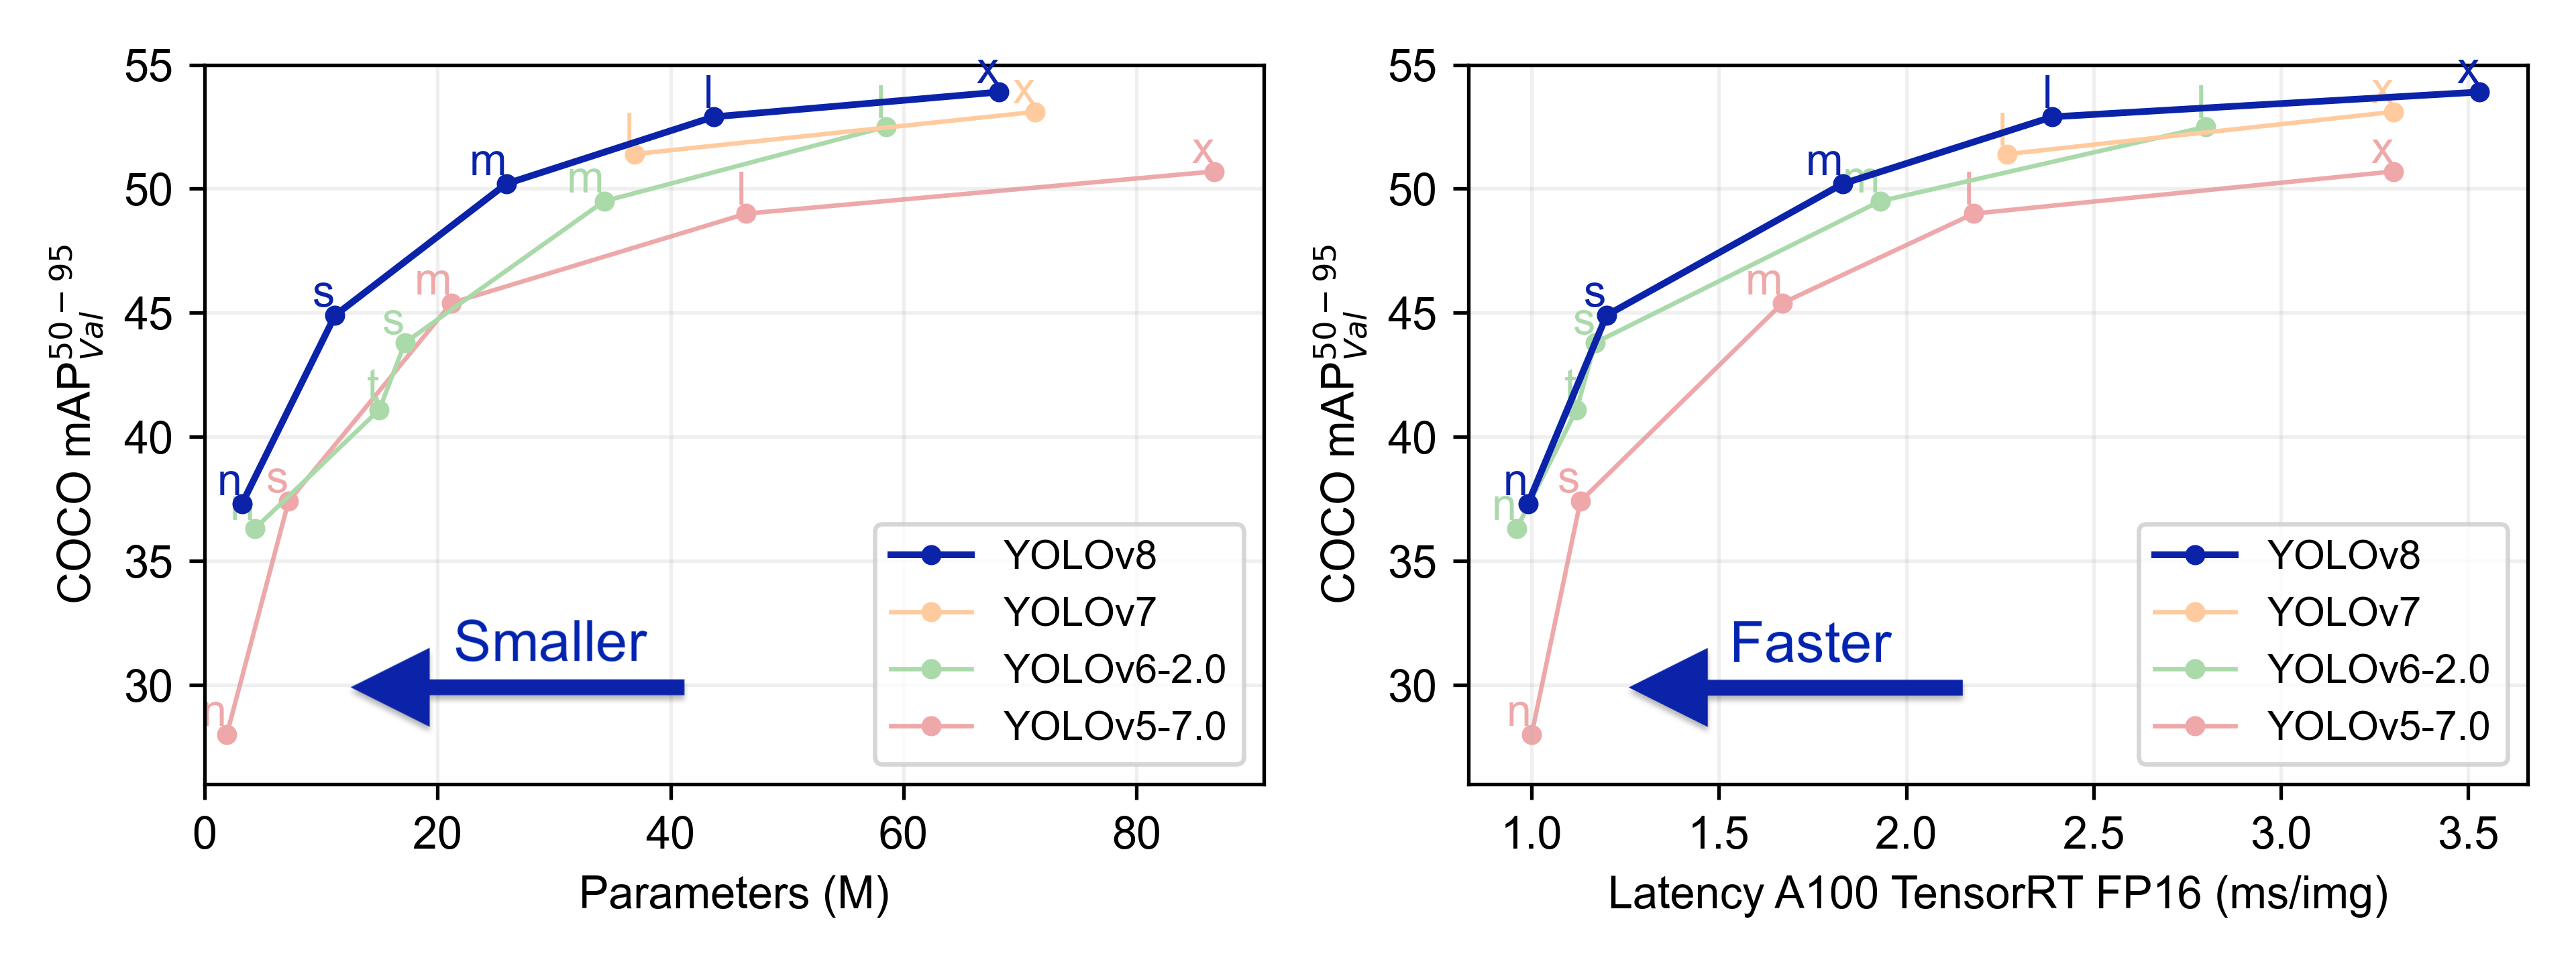
\includegraphics[width=150mm]{figures/yolo-comparison-plots.png}%
	\caption{YOLO parameters and latency comparison from \cite{yolov8}. Several other performance tests have shown that YOLOv8 outperforms YOLOv7 in terms of speed and accuracy.}%
	\label{YOLO comparison}%
\end{figure}%

\begin{enumerate}
	\item The switch to anchor-free detection head: The head module switched from anchor-based to anchor-free and adapted the current mainstream decoupled structure, separating the classification and detection heads. Anchor-free models directly predict an object's center instead of the offset from a known anchor box. Anchor-free detection reduces the number of box predictions, which speeds up the Non-Maximum Suppression (NMS) post-processing. Experimental results in \cite{detrs} show that with equivalent accuracy, YOLOv7 produces around three times more predicted boxes in comparison to YOLOv8. 
	\item The convolutional blocks undergo modifications to expedite the training process and improve gradient flow.
	\item Exploitation of Mosaic augmentation: Mosaic augmentation is the process of combining four images into a single mosaic image. This is done by resizing the four images, stitching them together, and then taking a random cutout. This technique enhances the model's ability to learn objects in new locations, partial occlusion, and with greater variation in surrounding pixels. However, it has been shown that using Mosaic augmentation throughout the entire training regime may have an adverse effect on prediction accuracy. Thus, YOLOv8 applies Mosaic augmentation only during training and turns it off before the last ten epochs. 
	\item YOLOv8 offers several developer-convenience features, from an easy-to-use CLI to a well-structured Python package.
\end{enumerate}

\subsection{Amodal Instance Segmentation}

Instance segmentation methods are restricted to detecting and segmenting the visible part of the objects, which can lead to poor performance in situations where objects are heavily occluded. Under such conditions, instances may be wholly missing, or the 2D bounding boxes and segments may be truncated, causing errors in downstream processes. In our case, these errors can affect the accuracy of 3D perception. To address the limitations of IS, amodal instance segmentation (AIS) techniques aim to predict the complete shapes of objects, including both visible and invisible parts. The full mask of an object is referred to as an amodal mask, while the visible mask is known as a modal or inmodal mask.

In this related work study, several survey AIS papers were consulted. Some of these papers are worth highlighting for reference. The Bilayer Convolutional Network (BCNet) \cite{bcnet} exploits a bilayer structure for occluding objects (occluders) and partially occluded instances (occludees). This approach naturally decouples the boundaries of both instances and considers the interaction between them during mask regression. AISFormer \cite{aisformer} enhances the extraction of the long-range dependency via transformer and explicitly models the complex coherence between occluder, visible, amodal, and invisible masks within an object's regions of interest by treating them as learnable queries. The self-supervised Amodal Video Object Segmentation (SaVos) \cite{savos} offers a solution for video amodal segmentation. SaVos leverages spatiotemporal consistency and dense object motion to explain away occlusion. Coarse-to-Fine Segmentation (C2F-Seg) \cite{c2fseg} model consists of two modules: a transformer-based module for predicting coarse amodal masks and a CNN-based refinement module for obtaining fine amodal masks. The paper of this model is published in ICCV 2023. The authors of C2F-seg conducted a comparison with several state-of-the-art models, including PCNet \cite{PCNet}, Mask R-CNN \cite{maskRCNN}, ORCNN \cite{ORCNN}, VRSP \cite{VRSP} and AISformer on the KINS and COCOA datasets and report the results in \Cref{tab:c2f_report}. This indicates that the C2F-Seg outperforms other state-of-the-art models on both datasets across average precision (AP) and mean intersection over union (mIoU) metrics.

\begin{table}[htbp]
	\centering
	{\scriptsize 
		\begin{tabular}{lrrrrr|rrrrr}
			\toprule
			\multirow{2}{*}{\textbf{Methods}} & \multicolumn{5}{c|}{\textbf{KINS}} & \multicolumn{5}{c}{\textbf{COCOA}} \\
			\cmidrule(r){2-6} \cmidrule(l){7-11}
			& \textbf{AP} & \textbf{AP@.5} & \textbf{AP@.75} & \textbf{mIoUfull} & \textbf{mIoUocc} & \textbf{AP} & \textbf{AP@.5} & \textbf{AP@.75} & \textbf{mIoUfull} & \textbf{mIoUocc} \\
			\midrule
			PCNet & 29.1 & 51.8 & 29.6 & 78.02 & 38.14 & --  & -- & -- & 76.91 & 20.34 \\
			Mask R-CNN & 30.0 & 54.5 & 30.1 & -- & -- & 28.0 & 53.7 & 25.4 & -- & -- \\
			ORCNN & 30.6 & 54.2 & 31.3 & -- & -- & 28.0 & 53.7 & 25.4 & -- & -- \\
			VRSP & 32.1 & 55.4 & 33.3 & 80.70 & 47.33  & 35.4 & 56.0 & 38.7 & 78.98 & 22.92 \\
			AISformer & 33.8 & 57.8 & 35.3 & 81.53 & 48.54 & 29.0 & 45.7 & 31.8 & 72.69 & 13.75 \\
			C2F-Seg & \textbf{36.5} & \textbf{58.2} & \textbf{37.0} & \textbf{82.22} & \textbf{53.60} & \textbf{36.6}& \textbf{57.0} & \textbf{38.5} & \textbf{80.28} & \textbf{27.71} \\
			\bottomrule
		\end{tabular}
		\caption{C2F-Se performance comparison on the KINS and COCOA reported by \cite{c2fseg}. The AP columns show AP@[.5:.95]}
		\label{tab:c2f_report}
	}
\end{table}

%\section{Coarse-to-Fine Amodal Segmentation with Shape Prior (C2F-seg)}  \label{sec:c2f}

\begin{figure}[htb]%
	\centering%
	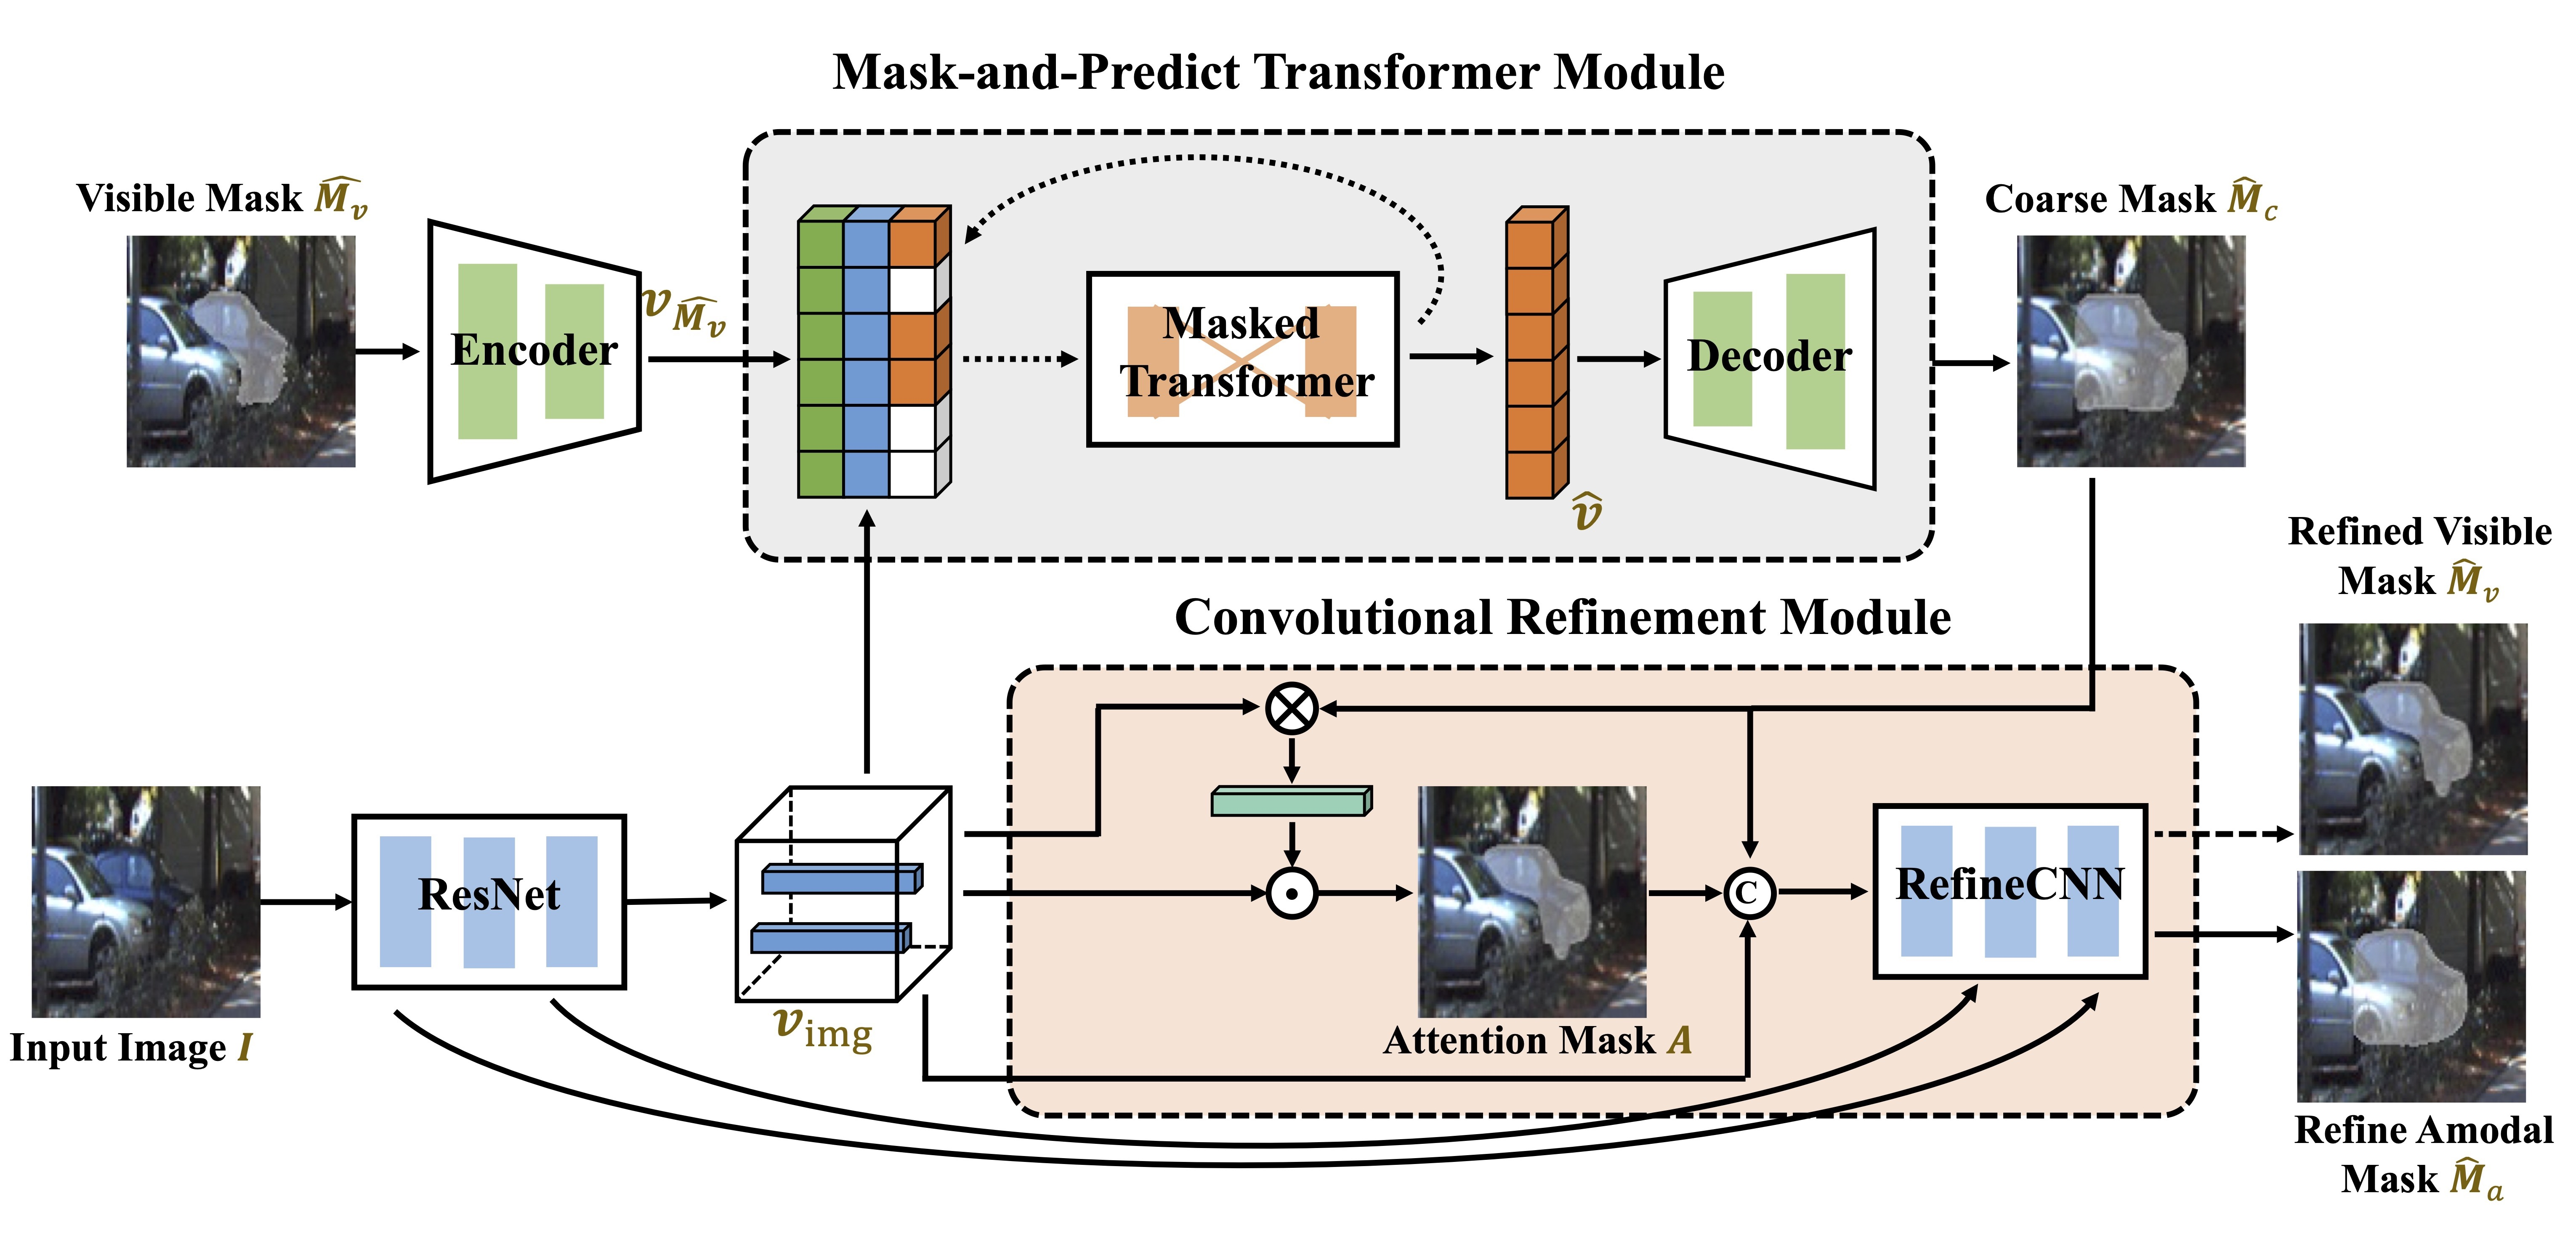
\includegraphics[width=130mm]{figures/C2F-Seg_arch.jpg}%
	\caption{The architecture of C2F-Seg taken from \cite{c2fseg}. The transformer module predicts coarse amodal masks from visual features and visible segments, while a convolutional refinement module refines the coarse predictions using visual features to generate final amodal segmentation mask predictions. Inference provides an estimate of the amodal mask based on input visible masks.}%
	\label{Fig:C2F_seg architecture}%
\end{figure}%

The following shows the Coarse-to-Fine Amodal Segmentation with Shape Prior (C2F-seg) model in more detail. C2F-Seg generates amodal segments progressively through two phases, as shown in \Cref{Fig:C2F_seg architecture}. The first coarse segmentation phase takes as inputs ResNet visual feature, vector-quantized visible segments, and ground-truth amodal segments masked in a high ratio. In this phase, a transformer is adopted and trained to reconstruct the masked tokens of the amodal segments. The reduction of learning space from pixel-level image space to low-dimension vector-quantized latent space makes the learning process easier and accelerates the inference process. The second refinement phase takes as inputs the coarse-predicted amodal segments from the first phase and the visual features. A semantic-inspired attention module is constructed as an initial stimulus, which gradually injects the visual features into the segments through convolution layers to finally arrive at a more precise amodal object segmentation. The learning of visible masks is used as an auxiliary task in training; inference only provides an estimate of the amodal mask based on the input of visible masks.

The C2F\_seg framework used for experiments in \cite{c2fseg} was implemented on the PyTorch platform and utilized pre-detected visible detections by AISFormer \cite{aisformer}. The model enlarges bounding boxes of visible regions twice and uses them to crop the image and mask inputs. The inputs are then all resized to 256×256, and various data augmentation techniques, including morphology dilation, erosion, and Gaussian blur, are applied.

